\section{Results}  \label{sec:results}
This section summarizes the results of this mapping review. The answer to each research question (from RQ1 to RQ12) is presented in tables and charts. The organization of extracted data follows the criteria defined in Section~\ref{sec:research_method}. 

\subsection{When and where have the studies been published? (RQ1)}\label{subsec:rq1}

Figure~\ref{fig:classification_by_publication_year} shows that research on bug report severity prediction in FLOSS is recent and active with a vast number of papers (22 out of 27 $\approx$ 81\%) published from 2014. Journals and conferences on information technology, mining software repositories, and software engineering seem to be more open to papers of bug report severity prediction (Table \ref{tab:papers_sources}). 

\begin{table}[h!]
  \centering
  \caption{Papers publication sources.}
  \begin{tabular}{@{}llr@{}} 
    \toprule
    \textbf{Paper source} & \textbf{Type} & \textbf{Reference} \\ 
    \midrule
    ACM Symposium on Applied Computing                 & Conference     & \cite{Zhang:2015}\\ 
    \midrule
    Advanced Science and Technology Letters \& Journal & Journal         & \cite{Jin:2016a}\\
    \midrule
    Asia-Pacific Software Engineering Conference         & Conference     & \cite{Yang:2012}\\
    \midrule
    Computational Science and Its Applications (ICCSA)     & Conference     & \cite{Meera:2014}\\
    \midrule
    Computer Software and Applications Conference         & Conference     & \cite{Yang:2014b}\\
    \midrule
    Contemporary Engineering Sciences                     & Journal         & \cite{Jin:2016b}\\
    \midrule
    Empirical Software Engineering                     & Journal         & \cite{Tian:2016}\\
    \midrule
    Futuristic Trends on Computational Analysis and Knowledge Management (ABLAZE) & Conference & \cite{Gujral:2015}\\
    \midrule
    Information and Software Technology                 & Journal         & \cite{Xia:2015}\\
    \midrule
    International Conference on Circuits, Controls, Communications and Computing (I4C) & Conference & \cite{Pushpalathas:2016}\\
    \midrule
    International Conference on Computer Science and Software Engineering         & Conference & \cite{Sabor:2016}\\
    \midrule
    International Conference on Information and Communication Systems (ICICS)     & Conference & \cite{Otoom:2016}\\
    \midrule
    International Conference on Software Engineering and Service Science        & Conference & \cite{Yang:2014a}\\
    \midrule
    International Information Institute                                 & Journal         & \cite{Jin:2016c}\\
    \midrule
    International Journal of Open Source Software and Process(IJOSSP)    & Journal         & \cite{Chaturvedi:2012}\\
    \midrule
    International MultiConference of Engineers and Computer Scientists     & Conference     & \cite{Choeikiwong:2016}\\
    \midrule
    Journal of Information \& Knowledge Management                         & Journal         & \cite{Singh:2017}\\
    \midrule
    Journal of Systems and Software                 & Journal     & \cite{Zhang:2016}\\
    \midrule
    Procedia Computer Science                     & Journal     & \cite{Sharma:2015}\\
    \midrule
    Software Engineering and Advanced Applications (SEAA) & Conference & \cite{Roy:2014}, \cite{Roy:2017}\\
    \midrule
    Symposium on Applied Computing (SAC)         & Conference & \cite{Yang:2017}\\
    \midrule
    Working Conference on Mining Software Repositories (MSR) & Conference & \cite{Lamkanfi:2010}, \cite{Lamkanfi:2011}, \cite{Valdivia:2014}, \cite{Saha:2015}\\
    \midrule
    Working Conference on Reverse Engineering     & Conference & \cite{Tian:2012} \\
    \bottomrule
  \end{tabular}
  \label{tab:papers_sources}
\end{table}

\subsection{What FLOSS are the most used as experimental target for bug report severity prediction (RQ2)?}\label{subsec:rq2_result}

Table \ref{tab:papers_by_floss} shows that most papers concentrated their focus on five FLOSS: Eclipse ($\approx$ 92\%), Mozilla ($\approx$ 70\%), Openoffice ($\approx$ 18\%), Netbeans ($\approx$ 14\%), and Gnome ($\approx$ 11\%). The detailing of each FLOSS including description, category, BTS, and URL is presented in Table \ref{tab:floss_descriptions}.

\begin{table}[h!]
  \vspace{0pt}
  \centering
  \captionsetup{type=table}
  \caption{Paper distribution by FLOSS.}
  \small
  \begin{tabular}{@{}lp{10cm}r@{}}
    \toprule
    \textbf{Project} & \textbf{References} & \textbf{Total}\\
    \midrule
    Eclipse & \cite{Lamkanfi:2010},\cite{Lamkanfi:2011},\cite{Tian:2012},\cite{Yang:2012},\cite{Chaturvedi:2012},\cite{Yang:2014b},\cite{Yang:2014a},\cite{Valdivia:2014},\cite{Roy:2014},\cite{Saha:2015},\cite{Zhang:2015},\cite{Sharma:2015},\cite{Xia:2015},\cite{Gujral:2015},\cite{Otoom:2016},\cite{Sabor:2016},\cite{Tian:2016},\cite{Zhang:2016},\cite{Jin:2016a},\cite{Choeikiwong:2016},\cite{Jin:2016b},\cite{Jin:2016c},\cite{Yang:2017},\cite{Singh:2017},\cite{Roy:2017},\cite{Lamkanfi:2011},\cite{Tian:2012},\cite{Yang:2012},\cite{Chaturvedi:2012},\cite{Yang:2014b},\cite{Yang:2014a},\cite{Valdivia:2014},\cite{Roy:2014},\cite{Saha:2015},\cite{Zhang:2015},\cite{Sharma:2015},\cite{Xia:2015},\cite{Gujral:2015},\cite{Otoom:2016},\cite{Sabor:2016},\cite{Tian:2016},\cite{Zhang:2016},\cite{Jin:2016a},\cite{Choeikiwong:2016},\cite{Jin:2016b},\cite{Jin:2016c},\cite{Yang:2017},\cite{Singh:2017},\cite{Roy:2017} & 25 \\
    \midrule
    Mozilla & \cite{Lamkanfi:2010},\cite{Tian:2012},\cite{Yang:2012},\cite{Chaturvedi:2012},\cite{Yang:2014b},\cite{Valdivia:2014},\cite{Meera:2014},\cite{Roy:2014},\cite{Zhang:2015},\cite{Xia:2015},\cite{Pushpalathas:2016},\cite{Otoom:2016},\cite{Tian:2016},\cite{Zhang:2016},\cite{Jin:2016a},\cite{Jin:2016b},\cite{Jin:2016c},\cite{Singh:2017},\cite{Roy:2017} & 19 \\
    \midrule
    Openoffice & \cite{Tian:2012},\cite{Valdivia:2014},\cite{Xia:2015},\cite{Tian:2016},\cite{Zhang:2016} & 5 \\
    \midrule
    Netbeans & \cite{Yang:2014b},\cite{Valdivia:2014},\cite{Xia:2015},\cite{Zhang:2016} & 4 \\
    \midrule
    Gnome & \cite{Lamkanfi:2010},\cite{Lamkanfi:2011},\cite{Chaturvedi:2012} & 3 \\
    \midrule
    Chromium & \cite{Valdivia:2014},\cite{Xia:2015} & 2 \\
    Freedesktop & \cite{Valdivia:2014},\cite{Xia:2015} & 2 \\
    \midrule
    GCC & \cite{Zhang:2016} & 1 \\
    \midrule
    Hibernate & \cite{Roy:2017} & 1 \\
    \midrule
    Spring & \cite{Roy:2017} & 1 \\
    \midrule
    Android & \cite{Yang:2017} & 1 \\
    \midrule
    JBoss & \cite{Yang:2017} & 1 \\
    \midrule
    Mongo-db & \cite{Roy:2017} & 1 \\
    \midrule
    WineHQ & \cite{Pushpalathas:2016} & 1 \\
    \bottomrule
  \end{tabular} 
  \label{tab:papers_by_floss}  
\end{table} 

Figure \ref{fig:distribution_by_floss} shows that most papers worked with FLOSS  related to Programming Tool ($\approx$ 92\%) and Application Software ($\approx$  74\%) categories. Moreover, it presents that 17 out of 27 ($\approx$ 62\%) papers worked with both categories. Figure \ref{fig:distribution_by_bts} highlights that all papers handled bug reports extracted from Bugzilla, and a just few papers from Google (3 out of 27 - $\approx$ 11\%) and Jira (2 out of 27 $\approx$ 7\%). Only one paper (Yang et al.\cite{Yang:2017}) investigated bug reports from three BTS.

\begin{table*}[h!]
  \centering
  \caption{FLOSS investigated in papers.}
  \begin{tabular}{@{}lllll@{}} 
    \toprule
    \textbf{Project} & \textbf{Description} & \textbf{Category} & \textbf{BTS} & \textbf{URL (As of \today)}\\ 
    \midrule
    Android        &  Mobile operating system     & System software & Google       & \url{https://issuetracker.google.com}            \\ 
    Chromium    &  Web browser                 & Application software & Google       & \url{https://www.chromium.org/issue-tracking}    \\ 
    Eclipse        &  Integrated Development Environment(IDE) &  Programming tool & Bugzilla  & \url{https://bugs.eclipse.org/bugs/}            \\ 
    FreeDesktop &  Base platform for desktop software on Linux and UNIX & Programing Tool & Bugzilla  & \url{https://bugs.freedesktop.org/}            \\ 
    GCC            &  C compiler                 & Programming tool & Bugzilla  & \url{https://gcc.gnu.org/bugzilla/}            \\ 
    Gnome        &  Desktop environment based on X Windows System & Application Software & Bugzilla  & \url{https://gcc.gnu.org/bugzilla/}            \\ 
    Hibernate    &  Object Relation Mapper(ORM) framework & Programming tool & Jira      & \url{https://hibernate.atlassian.net}            \\ 
    Jboss        &  Application server         & System software & Jira       & \url{https://issues.jboss.org/s}                \\ 
    Mongo-db    &  No-sql database             & System software & Jira       & \url{https://jira.mongodb.org/}                \\ 
    Mozilla        &  Internet tools             & Application software & Bugzilla     & \url{https://bugzilla.mozilla.org/}            \\ 
    Netbeans    &  Integrated Development Environment(IDE) & Programming tool    & Bugzilla  & \url{https://netbeans.org/bugzilla/}            \\ 
    OpenOffice    &  Office suite             & Application software & Bugzilla    & \url{https://bz.apache.org/ooo/}                \\ 
    Spring        &  JEE Framework             & Programming tool & Jira       & \url{https://jira.spring.io}                    \\ 
    WineHQ        &  Compatibility layer         & System software & Bugzilla  & \url{https://bugs.winehq.org/}                \\ 
    \bottomrule
  \end{tabular}
  \label{tab:floss_descriptions}
\end{table*}

%%%%
\begin{figure}[!htp]
  \begin{subfigure}{.94\textwidth}
    \centering
    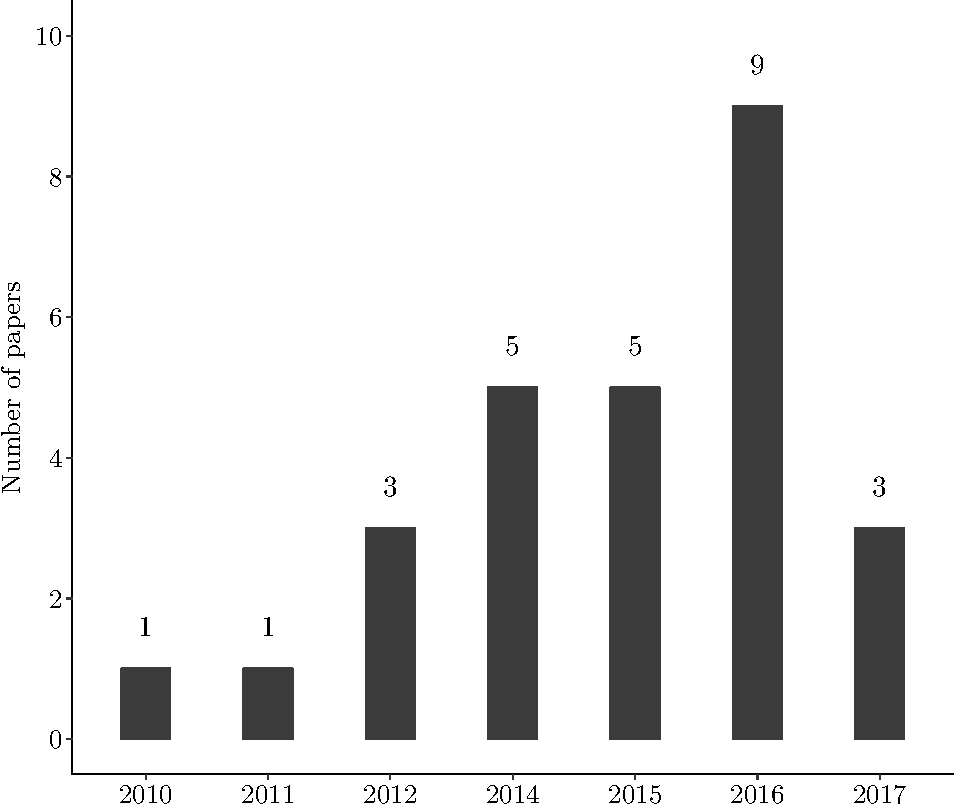
\includegraphics[width=0.5\textwidth]{figures/survey-summary-by-year-in-bar.pdf}
    \caption{}    
    \label{fig:classification_by_publication_year}
  \end{subfigure}\hfill
  %  \begin{subfigure}{.30\textwidth}
  %    \centering
  %    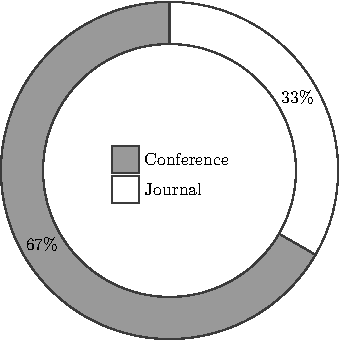
\includegraphics[width=0.9\textwidth]{figures/survey-summary-by-source-in-dnt.pdf}
  %    \caption{}
  %    \label{fig:classification_by_publication_source} 
  %  \end{subfigure}\hfill
  \begin{subfigure}{.49\textwidth}
    \centering
    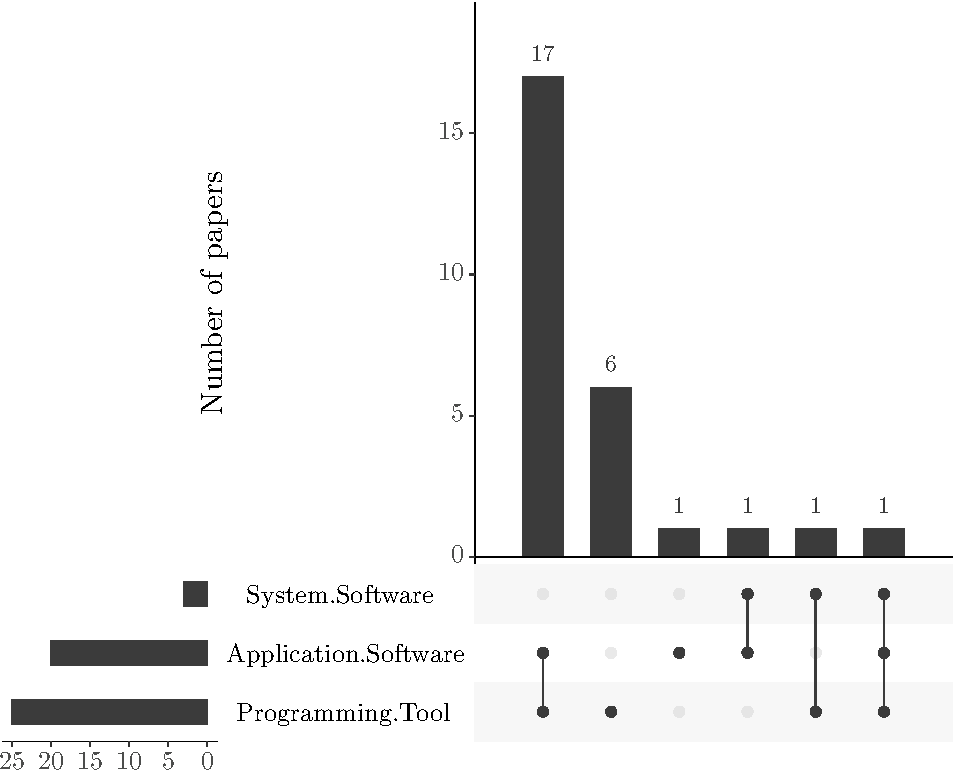
\includegraphics[width=\textwidth]{figures/distribution-by-floss-in-ups.pdf}
    \caption{}
    \label{fig:distribution_by_floss}
  \end{subfigure}\hfill
  \begin{subfigure}{.49\textwidth}
    \centering
    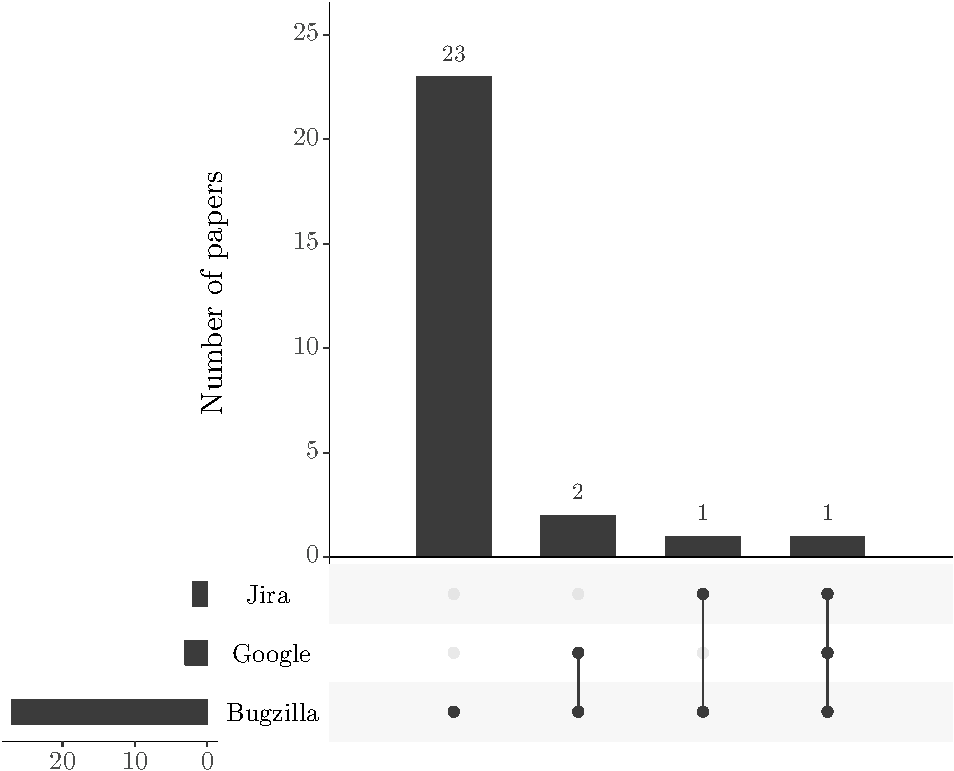
\includegraphics[width=\textwidth]{figures/distribution-by-bts-in-ups.pdf}
    \caption{}
    \label{fig:distribution_by_bts} 
  \end{subfigure}
  \caption{(a) Paper distribution by year (67\% published in conferences and 33\% in journals), (b) paper distribution by FLOSS (c) paper distribution by BTS.}
  \label{fig:rq1_classification}
\end{figure}
%%%%

\subsection{Was bug report severity prediction most addressed as either a fine-grained label  or coarse-grained label prediction problem (RQ3)?}\label{subsec:rq3_result}

Table~\ref{tab:prediction_problem_type_by_paper} shows that about the same fraction of papers addressed the bug report severity prediction as coarse-grained and fine-grained problem. Figure \ref{fig:distribution_by_problem-category_in_ups} shows that most papers  (10 out of 27 $\approx$ 37\%)  addressed the severity prediction as a problem of SNS category. Moreover, 8 out of 27 ($\approx$ 20\%) papers addressed it as a problem of the MC category and 5 out of 27 ($\approx$ 18.5\%) addressed a problem of the MCWD category. A few papers addressed a BNB (2 out of 27 $\approx$ 7\%) or an SNSWD (2 out of 27 $\approx$ 7\%) problem. No paper addressed more than one problem category.

\begin{table*}[h!]
  \vspace{30pt}
  \centering
  \captionsetup{type=table}
  \caption{Paper distribution by prediction problem.}
  \small
  \begin{tabular}{@{}lp{10cm}r@{}}
    \toprule
    \textbf{Problem} & \textbf{References} & \textbf{Total} \\
    \midrule
    Coarse-grained & \cite{Lamkanfi:2010},\cite{Lamkanfi:2011},\cite{Yang:2012},\cite{Yang:2014a},\cite{Roy:2014},\cite{Valdivia:2014},\cite{Sharma:2015},\cite{Gujral:2015},\cite{Xia:2015},\cite{Otoom:2016},\cite{Jin:2016a},\cite{Jin:2016b},\cite{Saha:2015},\cite{Jin:2016c} & 14 \\
    Fine-grained & \cite{Tian:2012},\cite{Chaturvedi:2012},\cite{Yang:2014b},\cite{Meera:2014},\cite{Zhang:2015},\cite{Pushpalathas:2016},\cite{Sabor:2016},\cite{Tian:2016},\cite{Zhang:2016},\cite{Choeikiwong:2016},\cite{Singh:2017},\cite{Yang:2017},\cite{Roy:2017} & 13 \\
    \bottomrule
  \end{tabular} 
  \label{tab:prediction_problem_type_by_paper}
\end{table*}

\subsection{What are the most common features used for bug report severity prediction (RQ4)?}\label{subsec:rq4_result}

Table~\ref{tab:features_descriptions} describes the features used for bug report severity prediction. Each feature in this table has a description, a category, an indicator of if the feature is computed from others, and an indicator of if the feature is available in Bugzilla, Jira, and Google.

\begin{table}[h!]
  \centering
  \spacebtrows{1.3}
  \caption{Feature descriptions.}
  \begin{tabular}{@{}lp{6cm}llllll@{}}
    \toprule
    \textbf{Feature}                      & \textbf{Description}                  & \textbf{Category}                     & \textbf{Calculated}?                  & \textbf{Bugzilla}                     & 
    \textbf{Jira}                         & 
    \textbf{Google}\\
    \midrule
    Attachments                  & Files (e.g., test cases or patches) attached to bugs.                                                                                                  & Qualitative Categorical            & No          &      Yes    &   No   & Yes\\
    Bug fix time                 & Time to fix a bug (Last Resolved Time - Opened Time).                                                                                                & Quantitative Continuous & Yes         &     Yes    &  Yes    &  Yes\\
    Bug id                       & Bug report identifier.                                                                                                                               & Quantitative Discrete  & No          &       Yes   &   Yes   & Yes\\
    CC list                      & A list of people who get mail when the bugs changes.                                                                                                 & Qualitative Categorical            & No          &       Yes   &    No  & Yes\\
    Comment                      & Textual content appearing in the comments of bug report.                                                                                             & Unstructured Text            & Yes         &       Yes   &    Yes  &  Yes\\
    Comment size                 & The number of word of all comments of a bug.                                                                                                         & Quantitative Discrete  & Yes         &      Yes    &    Yes  & Yes\\
    Complexity                   & Bug level of complexity based on bug fix time.                                                                                                       & Qualitative Ordinal           & Yes         &      Yes    &    Yes  & Yes\\
    Component                    & Each product is divided into different components (e.g., Core, Editor, and UI).                                                                      & Qualitative Categorical           & No          &     Yes     &   Yes   & Yes\\
    Description                  & Textual content appearing in the description field of the bug  report.                                                                               & Unstructured Text            & No          &   Yes       &  Yes    & Yes\\
    Description size             & The number of words in the description.                                                                                                              & Quantitative Discrete  & Yes         &      Yes    &   Yes   & Yes\\
    Importance                   & The importance of a bug is a combination of its priority and severity.                                                                               & Qualitative Discrete           & No          &     Yes     &    No  & No\\
    Number in CC list            & The number of developers in the CC list of the bug.                                                                                                  & Quantitative Discrete  & Yes         &     Yes     &   No   & Yes\\
    Number of comments           & Number of comments added to a bug by users.                                                                                                          & Quantitative Discrete  & Yes         &      Yes    &   Yes   & Yes\\
    Number of dependents         & Number of dependents of a bug report.                                                                                                                     & Quantitative Discrete  & Yes         &      Yes    &   Yes   & Yes\\
    Number of duplicates         & Number of duplicates of a bug report.                                                                                                                   & Quantitative Discrete  & Yes         &      No    &   No   & Yes\\
    Platform                     & Indicates the computing environment where the bug was found (e.g., Windows, GNU/Linux, and Android).                                            & Qualitative Categorical            & No          &   Yes       &  Yes    & Yes\\
    Priority                     & Priority should normally be set by the managers, maintainers or developers who plan to work, not by the one filling the bug or by outside observers. & Qualitative Ordinal            & No          &    Yes      &   Yes   & Yes\\
    Product                      & What general ``area” the bug belongs to (e.g., Firefox, Thunderbird, and Mailer).                                                                     & Qualitative Categorical           & No          &       Yes   &    Yes\footnotemark  & No\\
    Report length                & The content length of long description providing debugging information.                                                                              & Quantitative Discrete  & Yes         &     Yes     &    Yes  & Yes\\
    Reporter                     & The account of the user who created the bug report.                                                                                                  & Qualitative Categorical            & No          &       Yes   &   Yes   & Yes\\
    Reporter blocking experience & Counts the number of blocking bugs filed by reporter previous to this bug.                                                                           & Quantitative Discrete  & Yes         &   Yes       &   Yes   & No\\
    Reporter experience          & Counts the number of previous bug reports filed by the reporter.                                                                                     & Quantitative Discrete  & Yes         &  Yes        &  Yes    & No\\
    Reporter name                & Name of the developer or user that files the bug                                                                                                     & Qualitative Categorical           & No          &    Yes      &    Yes  & No\\
    Severity                     & Indicates how severe the problem is – from blocker (``application unusable”) to trivial (``minor cosmetic issue”).                                & Qualitative Ordinal            & No          &     Yes     &    Yes  & No\\
    Summary                      & A one-sentence summary of the problem.                                                                                                               & Unstructured Text            & No          &   Yes       &   Yes   & Yes\\
    Summary weight               & Score calculated using the information gain criterion.                                                                                                           & Quantitative Continuous  & Yes         &   Yes       &  Yes    & Yes\\
    \bottomrule
  \end{tabular}
  \label{tab:features_descriptions}
  
\end{table}
\footnotetext{In Jira, \textit{product} corresponds to \textit{project} field.}

As shown in Table~\ref{tab:features_by_papers}, most used features were \textit{summary} ($\approx$ 74\%) and \textit{description} ($\approx$ 70.37\%). Besides, a significant number of papers also reported using the features \textit{product} ($\approx$ 37\%) and \textit{component} ($\approx$ 33\%). Regarding data type of the features, unstructured text (26 out of 27 $\approx$ 96\%) was most used data type in the papers  (Figure \ref{fig:distribution_by_feature_category}). Only one paper (Meera et al.\cite{Meera:2014}) reported the use of features belonging to each data type presented in the chart.

\begin{table*}[h!]
  \vspace{30pt}
  \centering
  \captionsetup{type=table}
  \caption{Paper distribution by features.}
  \small
  \begin{tabular}{@{}lp{10cm}r@{}} 
    \toprule
    \textbf{Feature} & \textbf{References} & \textbf{Total} \\
    \midrule
    Summary & \cite{Lamkanfi:2010},\cite{Lamkanfi:2011},\cite{Tian:2012},\cite{Yang:2012},\cite{Chaturvedi:2012},\cite{Yang:2014b},\cite{Yang:2014a},\cite{Meera:2014},\cite{Saha:2015},\cite{Sharma:2015},\cite{Pushpalathas:2016},\cite{Otoom:2016},\cite{Tian:2016},\cite{Zhang:2016},\cite{Jin:2016a},\cite{Jin:2016b},\cite{Jin:2016c},\cite{Yang:2017},\cite{Singh:2017},\cite{Roy:2017} & 20 \\
    \midrule
    Description & \cite{Lamkanfi:2010},\cite{Tian:2012},\cite{Yang:2014b},\cite{Yang:2014a},\cite{Valdivia:2014},\cite{Roy:2014},\cite{Zhang:2015},\cite{Xia:2015},\cite{Gujral:2015},\cite{Pushpalathas:2016},\cite{Otoom:2016},\cite{Tian:2016},\cite{Sabor:2016},\cite{Zhang:2016},\cite{Jin:2016a},\cite{Jin:2016b},\cite{Jin:2016c},\cite{Yang:2017},\cite{Roy:2017} & 19 \\
    \midrule
    Product & \cite{Tian:2012},\cite{Yang:2014b},\cite{Valdivia:2014},\cite{Xia:2015},\cite{Pushpalathas:2016},\cite{Tian:2016},\cite{Zhang:2016},\cite{Jin:2016a},\cite{Jin:2016b},\cite{Jin:2016c} & 10 \\
    \midrule
    Component & \cite{Tian:2012},\cite{Yang:2014b},\cite{Valdivia:2014},\cite{Xia:2015},\cite{Pushpalathas:2016},\cite{Zhang:2016},\cite{Jin:2016a},\cite{Jin:2016b},\cite{Jin:2016c} & 9 \\
    \midrule
    Severity & \cite{Valdivia:2014},\cite{Xia:2015},\cite{Jin:2016a},\cite{Jin:2016b},\cite{Jin:2016c} & 5 \\
    \midrule
    Priority & \cite{Yang:2014b},\cite{Valdivia:2014},\cite{Meera:2014},\cite{Xia:2015} & 4 \\
    \midrule
    Reporter & \cite{Jin:2016a},\cite{Jin:2016b},\cite{Jin:2016c} & 3 \\
    \midrule
    Description size & \cite{Valdivia:2014},\cite{Xia:2015} & 2 \\
    \midrule
    Number in CC list & \cite{Valdivia:2014},\cite{Xia:2015} & 2 \\
    \midrule
    Reporter blocking experience & \cite{Valdivia:2014},\cite{Xia:2015} & 2 \\
    \midrule
    Reporter experience & \cite{Valdivia:2014},\cite{Xia:2015} & 2 \\
    \midrule
    Reporter name & \cite{Valdivia:2014},\cite{Xia:2015} & 2 \\
    \midrule
    Attachments & \cite{Yang:2014a} & 1 \\
    \midrule
    Bug fix time & \cite{Meera:2014} & 1 \\
    \midrule
    Bug Id & \cite{Choeikiwong:2016} & 1 \\
    \midrule
    CC list & \cite{Meera:2014} & 1 \\
    \midrule
    Comment & \cite{Valdivia:2014} & 1 \\
    \midrule
    Comment size & \cite{Xia:2015} & 1 \\
    \midrule
    Complexity & \cite{Meera:2014} & 1 \\
    \midrule
    Importance & \cite{Pushpalathas:2016} & 1 \\
    \midrule
    Number of comments & \cite{Meera:2014} & 1 \\
    \midrule
    Number of dependents & \cite{Meera:2014} & 1 \\
    \midrule
    Number of duplicates & \cite{Meera:2014} & 1 \\
    \midrule
    Platform & \cite{Xia:2015} & 1 \\
    \midrule
    Report length & \cite{Yang:2014a} & 1 \\
    \midrule
    Summary weight & \cite{Meera:2014} & 1 \\
    \bottomrule
  \end{tabular}
  \label{tab:features_by_papers}
\end{table*}


\subsection{What are the most common features selection methods employed for bug report severity prediction (RQ5)?}\label{subsec:rq5_result} 

Table~\ref{tab:features_selection_by_papers} shows that few papers ($\approx$ 40\%) use of a feature selection method for bug report severity prediction and remarkably all papers only used filter category methods.

\begin{table*}[h!]
  \centering
  \captionsetup{type=table}
  \caption{Paper distribution by feature selection methods.}
  \begin{tabular}{@{}llp{6.0cm}r@{}}
    \toprule
    \textbf{Method} & \textbf{Category} & \textbf{References} & \textbf{Total} \\
    \midrule
    Information Gain & Filter & \cite{Yang:2012},\cite{Chaturvedi:2012},\cite{Sharma:2015},\cite{Tian:2016},\cite{Roy:2017} & 5 \\
    \midrule
    Chi-Square & Filter & \cite{Yang:2012},\cite{Roy:2014},\cite{Sharma:2015} & 3 \\
    \midrule
    Correlation Coefficient & Filter & \cite{Yang:2012} & 1 \\
    \bottomrule
  \end{tabular} 
  \label{tab:features_selection_by_papers}
\end{table*}

\subsection{What are the most used text mining methods for bug report severity prediction (RQ6)?}\label{subsec:rq6_result}

As shown in Table~\ref{tab:papers_by_tm_models},  $\approx$ 74\% out of the papers used unigrams for feature vector extraction and $\approx$ 33\%  out of the papers used TF-IDF  for feature vector weighting. Regarding similarity/dissimilarity functions, $\approx$ 7\% reported using some function: one paper used BM25, one paper BM25ext, and another KL divergence.

Figure \ref{fig:distribution-by-tm-method-category} shows that most used text mining method (9 out of 15 $\approx$ 44\%) belongs to term category. Besides, only one paper (Yang et al.\cite{Yang:2017}) reported the use of text mining belonging to each category presented in the chart.

\begin{table*}[h!]
  \centering
  \captionsetup{type=table}
  \caption{Paper distribution by text mining models.}
  \small
  \begin{tabular}{@{}llp{10cm}r@{}}
    \toprule
    \textbf{Technique} & \textbf{Category} & \textbf{References} & \textbf{Total} \\
    \midrule
    \multicolumn{4}{c}{ \textit{Vector Extraction Models} } \\
    \midrule
    Unigrams & Character & \cite{Lamkanfi:2010},\cite{Lamkanfi:2011},\cite{Tian:2012},\cite{Yang:2012},\cite{Chaturvedi:2012},\cite{Yang:2014b},\cite{Yang:2014a},\cite{Roy:2014},\cite{Sharma:2015},\cite{Gujral:2015},\cite{Otoom:2016},\cite{Sabor:2016},\cite{Tian:2016},\cite{Zhang:2016},\cite{Jin:2016a},\cite{Choeikiwong:2016},\cite{Jin:2016b},\cite{Jin:2016c},\cite{Yang:2017},\cite{Singh:2017},\cite{Roy:2017} & 20 \\
    \midrule
    Bigrams & Character & \cite{Tian:2012},\cite{Roy:2014},\cite{Tian:2016},\cite{Zhang:2016} & 4 \\
    \midrule
    Topic model\footnotemark & Concept & \cite{Yang:2014b},\cite{Zhang:2015},\cite{Zhang:2016} & 3 \\
    \midrule
    \multicolumn{4}{c}{ \textit{Vector Weighting Models} } \\
    \midrule
    TF-IDF & Term & \cite{Lamkanfi:2011},\cite{Chaturvedi:2012},\cite{Roy:2014},\cite{Zhang:2015},\cite{Sharma:2015},\cite{Gujral:2015},\cite{Sabor:2016},\cite{Singh:2017},\cite{Roy:2017} & 9 \\
    \midrule
    TF & Term & \cite{Lamkanfi:2011},\cite{Yang:2012},\cite{Otoom:2016} & 3 \\
    \midrule
    Binary & Term & \cite{Lamkanfi:2011} & 1 \\
    \midrule
    \multicolumn{4}{c}{ \textit{Vector Similarity/Dissimilarity Functions} } \\
    \midrule
    BM25ext\footnotemark & Term & \cite{Zhang:2016} & 1 \\
    \midrule
    BM25 & Term & \cite{Tian:2012} & 1 \\
    KL divergence\footnotemark & Term & \cite{Yang:2014b} & 1 \\
    \bottomrule
  \end{tabular}
  \label{tab:papers_by_tm_models}
\end{table*}
\footnotetext[2]{Topic Model\cite{Zhang:2016} is a statistical model to identify ``topics" from a collection of documents. Each topic includes the
  topic terms which appear in the documents and each document may belong to one ou more topics.}
\footnotetext[3]{BM25ext\cite{Zhang:2016} is a extension of similarity function BM25. While BM25 computes the similarity of a short document with a long document, BM25ext computes the similarity between long documents.}
\footnotetext[4]{Kullback-Leibler(KL)\cite{Yang:2014b} divergence measures the difference between two probability over the same variable.}

\subsection{What are the most used machine learning algorithms for bug report severity prediction (RQ7)?}\label{subsec:rq7_result}

Table~\ref{tab:ml_algorithms_by_papers} presents that most papers used k-NN and NB ($\approx$ 44\%) and that NBM has also been used quite frequently ($\approx$ 40\%). As shown in Figure \ref{fig:distribution-by-ml-algorithm-category}, the majority of the papers used a probabilistic-based algorithm (21 out of 27 $\approx$ 77\%).  The figure also shows that 15 out of 27 papers ($\approx$ 55\%) used algorithms belonging to a ML algorithm single category.

\begin{table*}[h!]
  \centering
  \captionsetup{type=table}\textsl{}
  \caption{Papers distribution by ML algorithms}
  \begin{tabular}{@{}llp{10cm}r@{}}
    \toprule
    \textbf{Algorithm} & \textbf{Category} & \textbf{References} & \textbf{Total} \\
    \midrule
    KNN & Distance & \cite{Lamkanfi:2011},\cite{Tian:2012},\cite{Yang:2014b},\cite{Valdivia:2014},\cite{Meera:2014},\cite{Zhang:2015},\cite{Gujral:2015},\cite{Sabor:2016},\cite{Tian:2016},\cite{Zhang:2016},\cite{Choeikiwong:2016},\cite{Singh:2017} & 12 \\
    \midrule
    NB & Probabilistic & \cite{Lamkanfi:2010},\cite{Lamkanfi:2011},\cite{Chaturvedi:2012},\cite{Yang:2014b},\cite{Valdivia:2014},\cite{Meera:2014},\cite{Roy:2014},\cite{Saha:2015},\cite{Zhang:2015},\cite{Otoom:2016},\cite{Choeikiwong:2016},\cite{Singh:2017} & 12 \\
    \midrule
    NBM\footnotemark & Probabilistic & \cite{Lamkanfi:2011},\cite{Yang:2012},\cite{Yang:2014a},\cite{Zhang:2015},\cite{Sharma:2015},\cite{Gujral:2015},\cite{Tian:2016},\cite{Jin:2016a},\cite{Jin:2016b},\cite{Jin:2016c},\cite{Yang:2017} & 11 \\
    \midrule
    SVM & Otimization & \cite{Lamkanfi:2011},\cite{Chaturvedi:2012},\cite{Meera:2014},\cite{Tian:2016},\cite{Choeikiwong:2016},\cite{Singh:2017},\cite{Roy:2017} & 7 \\
    \midrule
    Random Forest & Ensemble & \cite{Chaturvedi:2012},\cite{Valdivia:2014},\cite{Xia:2015},\cite{Otoom:2016},\cite{Choeikiwong:2016} & 5 \\
    \midrule
    C4.5\footnotemark & Searching & \cite{Chaturvedi:2012},\cite{Valdivia:2014},\cite{Pushpalathas:2016} & 3 \\
    \midrule
    Bagging & Ensemble & \cite{Xia:2015},\cite{Pushpalathas:2016} & 2 \\
    \midrule
    Decision Tree & Searching & \cite{Tian:2016},\cite{Choeikiwong:2016} & 2 \\
    \midrule
    AdaBoost & Ensemble & \cite{Otoom:2016} & 1 \\
    \midrule
    Functional Tree & Searching & \cite{Otoom:2016} & 1 \\
    \midrule
    Random Tree & Ensemble & \cite{Otoom:2016} & 1 \\
    \midrule
    RBF Networks & Optimization & \cite{Otoom:2016} & 1 \\
    \midrule
    RIPPER\footnotemark & Other & \cite{Chaturvedi:2012} & 1 \\
    \midrule
    Zero-R\footnotemark & Other & \cite{Valdivia:2014} & 1 \\
    \bottomrule
  \end{tabular}
  \label{tab:ml_algorithms_by_papers}
\end{table*}
\footnotetext[5]{Näive Bayes Multinomial (NBM)\cite{Lamkanfi:2011} is similar to Näive Bayes. However, the output class is not only determined by presence or absence of term, but NBM also uses the number of occurrences of the terms to decide.}
\footnotetext[6]{C4.5\cite{Valdivia:2014} is an algorithm used to generate a decision tree which follows a greedy divide and conquer strategy in training step.}
\footnotetext[7]{Bagging Ensemble\cite{Xia:2015} uses multiple learning algorithms to obtain better predictive performance that could be received from any of the constituent learning algorithms alone. This approach involves having each model in the ensemble vote with equal weight. To promote model variance, bagging trains each model in the ensemble using a randomly drawn subset of the training set.}
\footnotetext[8]{AdaBoost\cite{Otoom:2016} is an ensemble algorithm that attempts to produce a very accurate classification rule by combining moderately inaccurate weak classifiers.}
\footnotetext[9]{Functional Tree\cite{Otoom:2016} is a classification tree that could have logistic regression function at the inner nodes and or leaves.}
\footnotetext[10]{Random Tree\cite{Otoom:2016} is an ensemble classifier that consists of directed graphs build with a random process.}
\footnotetext[11]{Radial Basis Function (RBF) Neural Network\cite{Marsland:2014} is a neural network that consists of input nodes connected by weights to a set of RBF neuron, which fire proportionally to the distance between the input and the neuron in weight space. RBF is a real-valued function whose value depends only on the distance from the origin.}
\footnotetext[12]{RIPPER\cite{Menzies:2008} is a rule-based classifier that builds a set of rules that identify the classes while minimizing the amount of error. The error is defined by the number of training examples misclassified by the regulations.}
\footnotetext[13]{Zero-R\cite{Valdivia:2014} is the simplest classifier which always predicts the majority class in training set. It is commonly employed for determining a baseline performance as a benchmark for other methods.}

\begin{figure}[!htp]
  \begin{subfigure}{.49\textwidth}
    \centering
    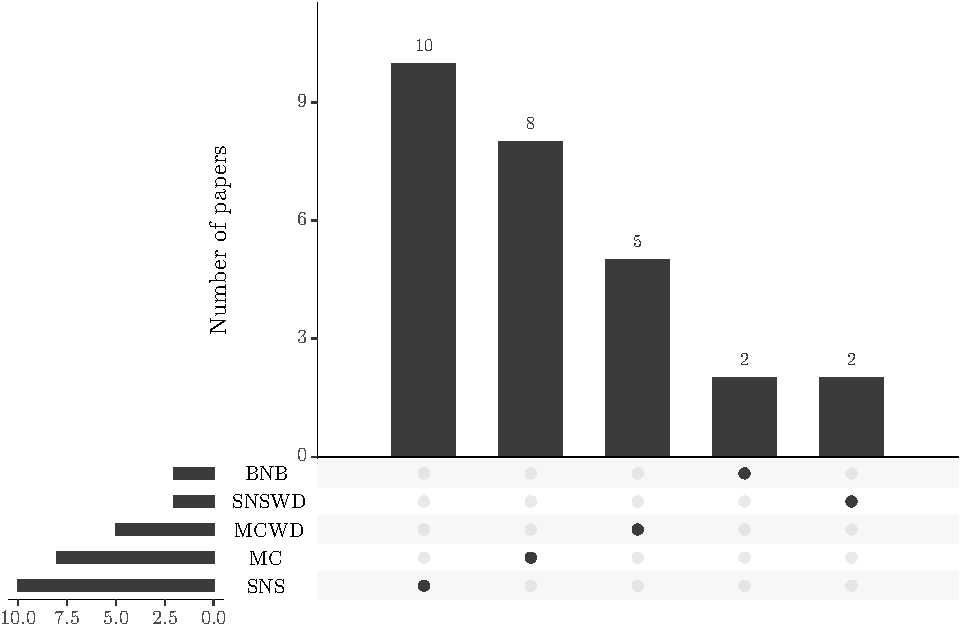
\includegraphics[width=\textwidth]{figures/distribution-by-problem-category-in-ups.pdf}
    \caption{}
    \label{fig:distribution_by_problem-category_in_ups}
  \end{subfigure}\hfill
  \begin{subfigure}{.49\textwidth}
    \centering
    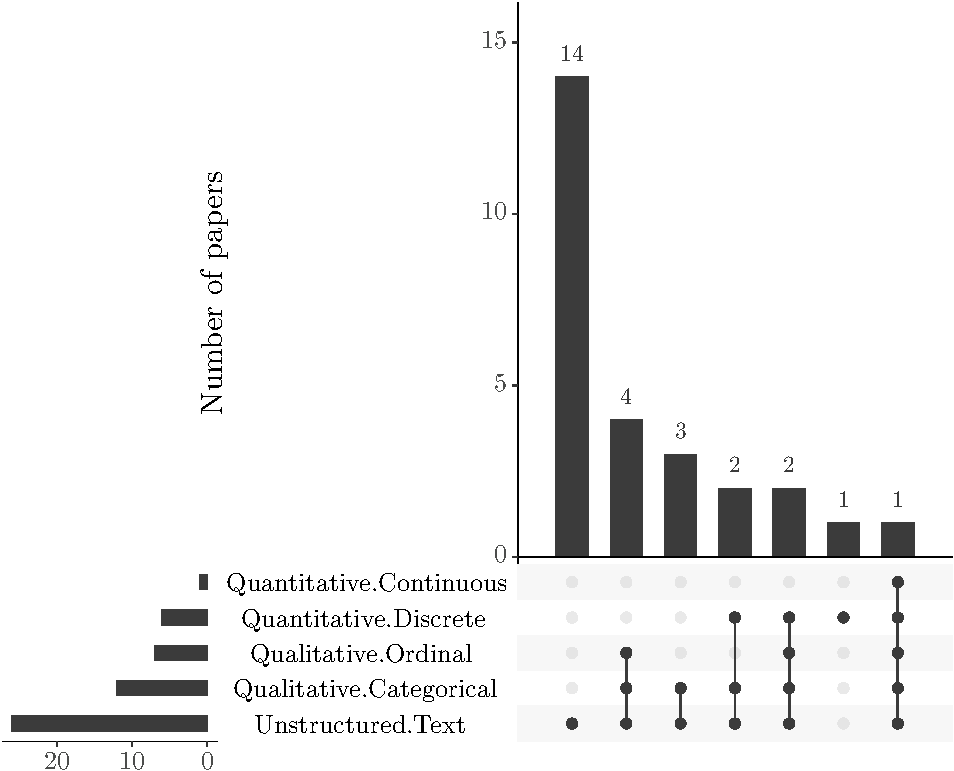
\includegraphics[width=\textwidth]{figures/distribution-by-feature-category-in-ups.pdf}
    \caption{}
    \label{fig:distribution_by_feature_category} 
  \end{subfigure}\hfill
  \begin{subfigure}{.49\textwidth}
    \centering
    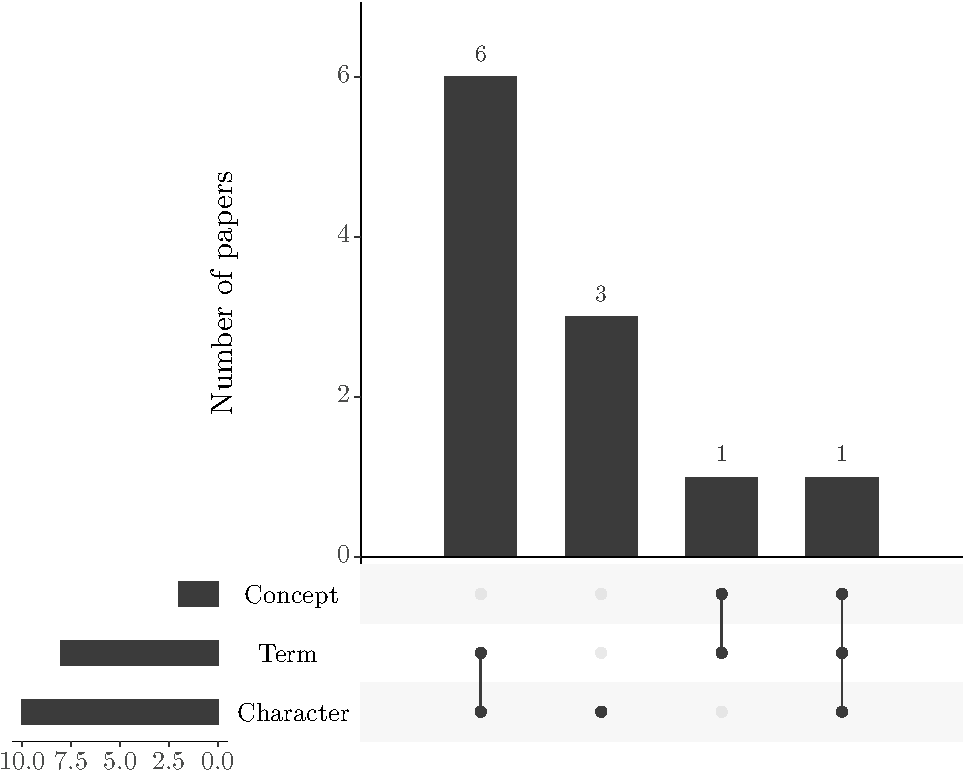
\includegraphics[width=\textwidth]{figures/distribution-by-tm-method-category-in-ups.pdf}
    \caption{}
    \label{fig:distribution-by-tm-method-category}
  \end{subfigure}\hfill
  \begin{subfigure}{.49\textwidth}
    \centering
    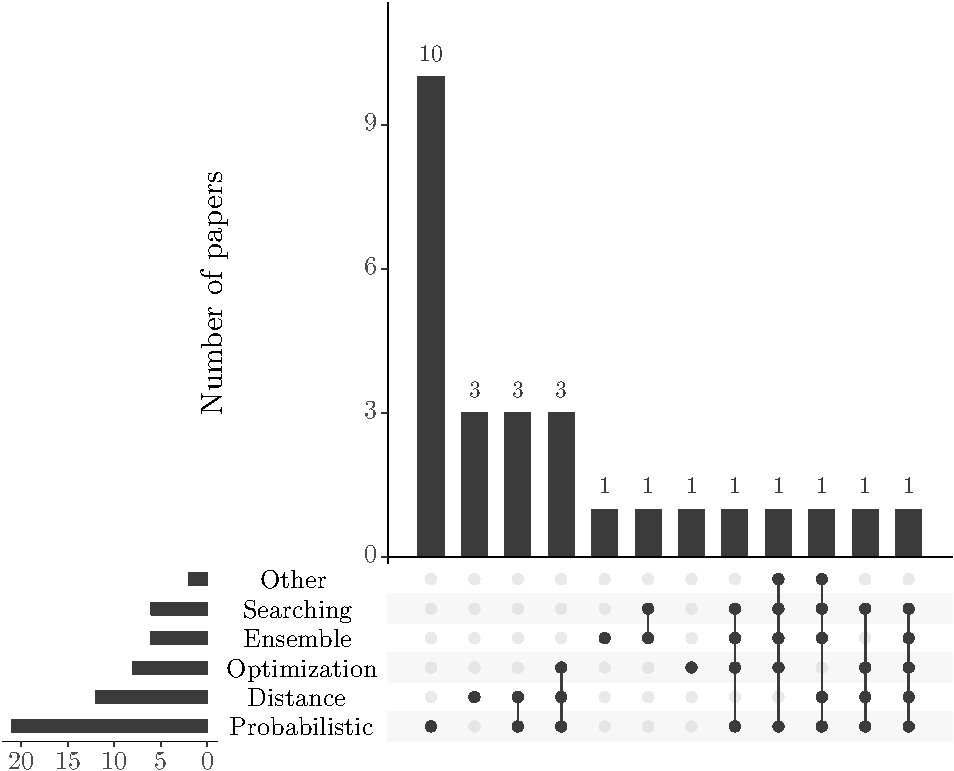
\includegraphics[width=\textwidth]{figures/distribution-by-ml-algorithm-category-in-ups.pdf}
    \caption{}
    \label{fig:distribution-by-ml-algorithm-category} 
  \end{subfigure}
  \caption{(a) Paper distribution by prediction problem category, (b) paper distribution by feature data category, (c) paper distribution by text mining method category (d) paper distribution by ML algorithm categories.}
  \label{fig:rq3_4_6_7_charts}
\end{figure}

\subsection{What are the measures used to evaluate ML algorithms performance for bug report severity prediction (RQ8)?}\label{subsec:rq8_result}

Most papers evaluated the ML model accuracy in bug report severity prediction using three measures based on the confusion matrix (Table~\ref{tab:evaluation_measures_by_papers}): precision ($\approx$ 77\%), recall ($\approx$ 70\%), and f-measure ($\approx$ 66\%). The majority of the used measures are of the single class category (21 out of 27 $\approx$ 70\%), as shown in Figure \ref{fig:distribution_by_evaluation_measure_category}. Only one paper (Roy et al.\cite{Roy:2014}) investigated all four categories of measures presented in the chart.

\begin{table*}[h!]
  \centering
  \captionsetup{type=table}\textsl{}
  \caption{Papers distribution by evaluation measures.}
  \begin{tabular}{@{}llp{8cm}r@{}}
    \toprule
    \textbf{Measure} & \textbf{Category} & \textbf{References} & \textbf{Total} \\
    \midrule
    Precision & Single Class & \cite{Lamkanfi:2010},\cite{Tian:2012},\cite{Chaturvedi:2012},\cite{Yang:2014b},\cite{Valdivia:2014},\cite{Meera:2014},\cite{Roy:2014},\cite{Zhang:2015},\cite{Sharma:2015},\cite{Xia:2015},\cite{Gujral:2015},\cite{Pushpalathas:2016},\cite{Sabor:2016},\cite{Zhang:2016},\cite{Jin:2016a},\cite{Choeikiwong:2016},\cite{Jin:2016b},\cite{Jin:2016c},\cite{Yang:2017},\cite{Singh:2017},\cite{Roy:2017} & 21 \\
    \midrule
    Recall & Single Class & \cite{Lamkanfi:2010},\cite{Tian:2012},\cite{Chaturvedi:2012},\cite{Yang:2014b},\cite{Valdivia:2014},\cite{Meera:2014},\cite{Roy:2014},\cite{Zhang:2015},\cite{Xia:2015},\cite{Pushpalathas:2016},\cite{Sabor:2016},\cite{Zhang:2016},\cite{Jin:2016a},\cite{Choeikiwong:2016},\cite{Jin:2016b},\cite{Jin:2016c},\cite{Yang:2017},\cite{Singh:2017},\cite{Roy:2017} & 19 \\
    \midrule
    F-measure & Single Class & \cite{Lamkanfi:2010},\cite{Tian:2012},\cite{Chaturvedi:2012},\cite{Yang:2014b},\cite{Valdivia:2014},\cite{Meera:2014},\cite{Roy:2014},\cite{Zhang:2015},\cite{Xia:2015},\cite{Sabor:2016},\cite{Zhang:2016},\cite{Jin:2016a},\cite{Choeikiwong:2016},\cite{Jin:2016b},\cite{Jin:2016c},\cite{Yang:2017},\cite{Singh:2017},\cite{Roy:2017} & 18 \\
    \midrule
    Accuracy & Multi-Class & \cite{Chaturvedi:2012},\cite{Yang:2014b},\cite{Valdivia:2014},\cite{Meera:2014},\cite{Roy:2014},\cite{Saha:2015},\cite{Sharma:2015},\cite{Gujral:2015},\cite{Pushpalathas:2016},\cite{Otoom:2016},\cite{Singh:2017} & 11 \\
    \midrule
    AUC & Summary & \cite{Lamkanfi:2010},\cite{Lamkanfi:2011},\cite{Yang:2012},\cite{Yang:2014a},\cite{Roy:2014} & 5 \\
    \midrule
    ROC & Graphical & \cite{Lamkanfi:2010},\cite{Roy:2014} & 2 \\
    \midrule
    MRR\footnotemark & Single Class & \cite{Yang:2014b},\cite{Zhang:2016} & 2 \\
    \midrule
    Effectiveness Ratio\footnotemark & Single Class & \cite{Xia:2015} & 1 \\
    \midrule
    Krippendorff's Alpha Reliability\footnotemark & Single Class & \cite{Tian:2016} & 1 \\
    \bottomrule
  \end{tabular}
  \label{tab:evaluation_measures_by_papers}
\end{table*}
\footnotetext[14]{Mean Reciprocal Rank (MRR)\cite{Zhou:2012} is the average of reciprocal ranks of results of a set of questions. A reciprocal rank of a question is the multiplicative inverse of the rank of the first correct answer.}
\footnotetext[15]{Effectiveness Ratio\cite{Xia:2015} is a cost-effectiveness measure, which evaluates prediction performance given a cost limit.}
\footnotetext[16]{Krippendorff's Alpha Coefficient\cite{Tian:2016} is a statistical measure of the agreement achieved when coding a set o units analysis of values of a variable.}

\subsection{Which sampling techniques are applied most frequently to generate more reliable predictive performance estimates in severity prediction of a bug report (RQ9)?}\label{subsec:rq9_result}

Most papers shown in Table~\ref{tab:sampling_methods_by_papers} applied 10-Fold CV ($\approx$ 66\%) to generate more reliable effectiveness estimates. Figure \ref{fig:distribution_by_sampling_method_category} displays that the majority of those papers (14 out of 15 $\approx$ 93\%) employed a simple resampling method. Also, only one paper (Otoom et al.\cite{Otoom:2016}) investigated both non-resampling and simple resampling methods for bug report severity prediction. 

\begin{table*}[h!]
  \centering
  \captionsetup{type=table}
  \caption{Paper distribution by sampling methods.}
  \small
  \begin{tabular}{@{}llp{8cm}r@{}}
    \toprule
    \textbf{Method} & \textbf{Category} & \textbf{References} & \textbf{Total} \\
    \midrule
    10-Fold CV & Simple Re-sampling & \cite{Lamkanfi:2011},\cite{Yang:2012},\cite{Chaturvedi:2012},\cite{Yang:2014a},\cite{Xia:2015},\cite{Pushpalathas:2016},\cite{Otoom:2016},\cite{Jin:2016b},\cite{Yang:2017},\cite{Roy:2017} & 10 \\
    \midrule
    Stratified 10-Fold CV\footnotemark & Simple Re-sampling & \cite{Valdivia:2014},\cite{Roy:2014},\cite{Singh:2017} & 3 \\
    \midrule
    SMOTE\footnotemark & Simple Re-sampling & \cite{Xia:2015},\cite{Choeikiwong:2016} & 2 \\
    \midrule
    Hold-out & No Re-sampling & \cite{Otoom:2016} & 1 \\
    \midrule
    03-Fold CV & Simple Re-sampling & \cite{Choeikiwong:2016} & 1 \\
    \midrule
    05-Fold CV & Simple Re-sampling & \cite{Sharma:2015} & 1 \\
    \bottomrule
  \end{tabular} 
  \label{tab:sampling_methods_by_papers}
\end{table*}
\footnotetext[17]{Stratified k-fold CV\cite{Japkowicz:2011} is a k-fold CV variation, which ensures that class distribution is respected in the training and testing sets created at every fold.}
\footnotetext[18]{Synthetic Minority Oversampling TEchnique (SMOTE)\cite{Chawla:2002} is an sampling approach in which the minority class is over-sampled by creating ``synthetic" examples rather than by over-sampling with replacement.}

\subsection{Which statistical tests were used to compare the performance between two or more ML algorithms for bug report severity prediction (RQ10)?}\label{subsec:rq10}

As shown in Table~\ref{tab:statistical_test_type_by_papers}, most of the papers used  Wilcoxon Signed Rank Test (8 out of 27 $\approx$ 29\%) and t-test (7 out of 27 - $\approx$ 26\%) to compare the performance of ML algorithms. Figure \ref{fig:distribution-by-statistical-method-category} calls attention that only ten papers ($\approx$ 37\%) reported using any statistical test in their experiments to bug report severity prediction. The figure also shows that most of these papers  (8 out of 10 $\approx$ 80\%) applied a non-parametric test, and 5 out of 10 (50\%) papers employed both parametric and non-parametric tests.  

\begin{table*}[h!]
  \centering
  \captionsetup{type=table}
  \caption{Paper distribution by statistical tests.}
  \begin{tabular}{@{}llp{6cm}r@{}}
    \toprule
    \textbf{Test} & \textbf{Category} & \textbf{References} & \textbf{Total} \\
    \midrule
    Wilcoxon signed rank test & Non-parametric & \cite{Yang:2014b},\cite{Valdivia:2014},\cite{Zhang:2015},\cite{Xia:2015},\cite{Zhang:2016},\cite{Jin:2016b},\cite{Yang:2017},\cite{Singh:2017} & 8 \\
    \midrule
    T-test & Parametric & \cite{Yang:2014b},\cite{Zhang:2015},\cite{Zhang:2016},\cite{Choeikiwong:2016},\cite{Jin:2016b},\cite{Yang:2017},\cite{Roy:2017} & 7 \\
    \midrule
    Proportion test & Parametric & \cite{Roy:2017} & 1 \\
    \midrule
    Shapiro-Wilk test & Parametric & \cite{Yang:2017} & 1 \\
    \bottomrule
  \end{tabular} 
  \label{tab:statistical_test_type_by_papers}
\end{table*}

\subsection{Which software tools were used to run bug report severity prediction experiments (RQ11)?}\label{subsec:rq11} 

Most of the papers listed in Table~\ref{tab:software_tools_used_in_papers} used RapidMiner (5 out of 18 $\approx$ 27\%) to run their experiments. However, Figure \ref{fig:distribution_by_software_tool_category} presents a strong predominance of FLOSS over CSS, 13 out of 18  papers ($\approx$ 61\%) executed  FLOSS to perform their experiments. The figure also shows that no paper used both CSS and FLOSS.

\begin{table*}[h!]
  \centering
  \captionsetup{type=table}
  \caption{Paper distribution by software tools.}
  \begin{tabular}{@{}llp{6cm}r@{}}
    \toprule
    \textbf{Tool} & \textbf{Category} & \textbf{References} & \textbf{Total} \\
    \midrule
    RapidMiner & CSS & \cite{Chaturvedi:2012},\cite{Meera:2014},\cite{Sharma:2015},\cite{Gujral:2015},\cite{Singh:2017} & 5 \\
    \midrule
    WEKA & FLOSS & \cite{Lamkanfi:2011},\cite{Xia:2015},\cite{Pushpalathas:2016},\cite{Tian:2016} & 4 \\
    \midrule
    R & FLOSS & \cite{Yang:2014b},\cite{Zhang:2015},\cite{Yang:2017} & 3 \\
    \midrule
    NLTK & FLOSS & \cite{Roy:2014},\cite{Zhang:2016},\cite{Jin:2016b} & 3 \\
    \midrule
    Statisca & CSS & \cite{Chaturvedi:2012},\cite{Meera:2014} & 2 \\
    \midrule
    TMT & FLOSS & \cite{Yang:2014b},\cite{Zhang:2016} & 2 \\
    \midrule
    OpenNLP & FLOSS & \cite{Tian:2012} & 1 \\
    \midrule
    WordNet & FLOSS & \cite{Roy:2014} & 1 \\
    \midrule
    Ruby & FLOSS & \cite{Lamkanfi:2010} & 1 \\
    \midrule
    WVTool & FLOSS & \cite{Yang:2012} & 1 \\
    \midrule
    CoreNLP & FLOSS & \cite{Yang:2017} & 1 \\
    \bottomrule
  \end{tabular} 
  \label{tab:software_tools_used_in_papers}
\end{table*}

\begin{figure}[!htp]
  \begin{subfigure}{.49\textwidth}
    \centering
    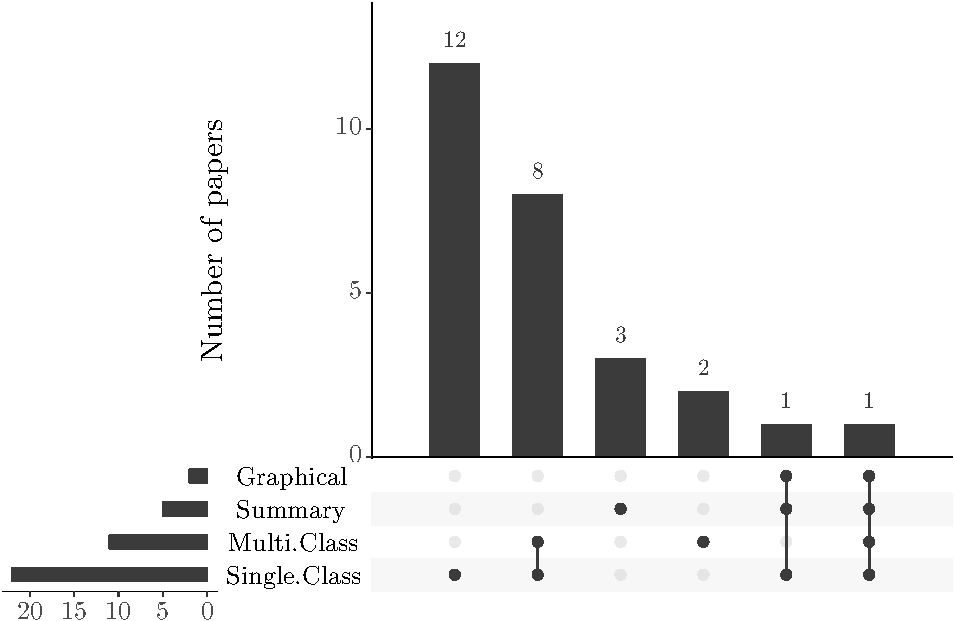
\includegraphics[width=\textwidth]{figures/distribution-by-evaluation-measure-category-in-ups.pdf}
    \caption{}
    \label{fig:distribution_by_evaluation_measure_category}
  \end{subfigure}\hfill
  \begin{subfigure}{.49\textwidth}
    \centering
    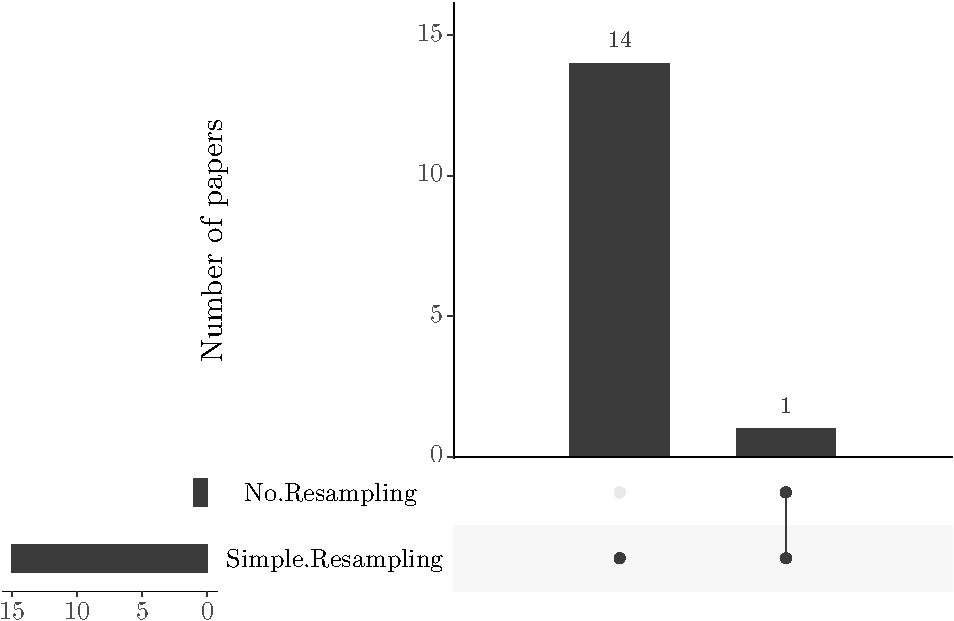
\includegraphics[width=\textwidth]{figures/distribution-by-sampling-method-category-in-ups.pdf}
    \caption{} 
    \label{fig:distribution_by_sampling_method_category}
  \end{subfigure}\hfill
  \begin{subfigure}{.49\textwidth}
    \centering
    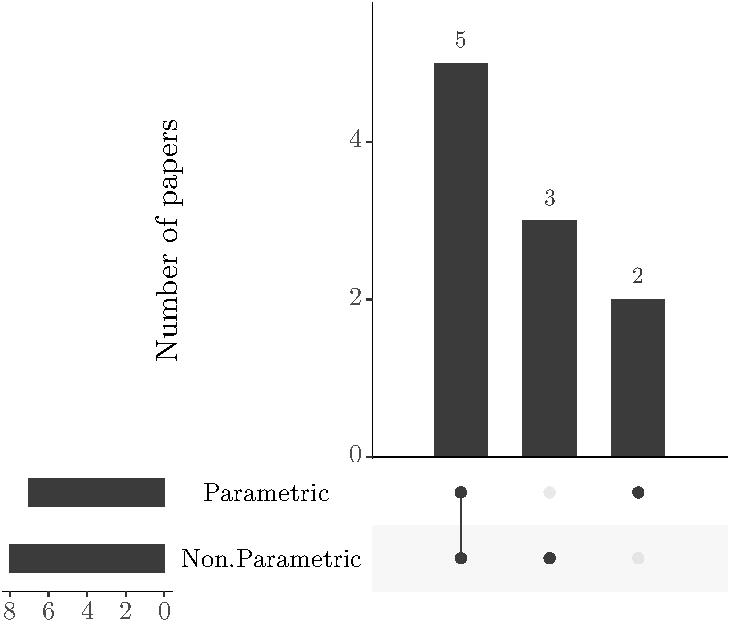
\includegraphics[width=\textwidth]{figures/distribution-by-statistical-method-category-in-ups.pdf}
    \caption{}
    \label{fig:distribution-by-statistical-method-category}
  \end{subfigure}\hfill
  \begin{subfigure}{.49\textwidth}
    \centering
    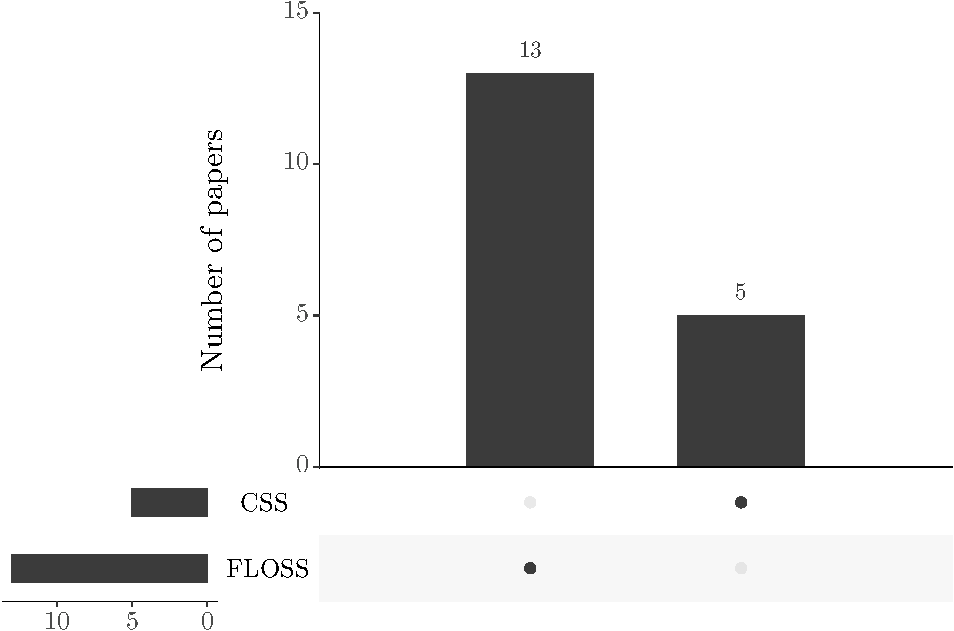
\includegraphics[width=\textwidth]{figures/distribution-by-software-tool-category-in-ups.pdf}
    \caption{}
    \label{fig:distribution_by_software_tool_category} 
  \end{subfigure}
  \caption{(a) Paper distribution by evaluate measure categories, (b) paper distribution by sampling method categories, (c) paper distribution by statistical test categories, and (d) paper distribution by software tool categories.}
  \label{fig:rq8_9_10_11_charts}
\end{figure}
%%%%
\subsection{Which solution types were proposed for bug report severity prediction problem (RQ12)?}\label{subsec:rq12}

Most of the papers (26 out of 27 $\approx$ 93\%) provided offline solutions (Table~\ref{tab:solutions_types_by_papers}). Just one paper (Tian et al. \cite{Tian:2012}) presented an online solution.

\begin{table*}[!htbp]
  \centering
  %\spacebtrows{1.3}
  \caption{Solution types proposed in selected papers.}
  \begin{tabular}{@{}lp{6cm}r@{}}
    \toprule
    Tool & References & Total \\
    \midrule
    offline & \cite{Lamkanfi:2010},\cite{Lamkanfi:2011},\cite{Yang:2012},\cite{Chaturvedi:2012},\cite{Yang:2014b},\cite{Yang:2014a},\cite{Valdivia:2014},\cite{Meera:2014},\cite{Roy:2014},\cite{Saha:2015},\cite{Zhang:2015},\cite{Sharma:2015},\cite{Xia:2015},\cite{Gujral:2015},\cite{Pushpalathas:2016},\cite{Otoom:2016},\cite{Sabor:2016},\cite{Tian:2016},\cite{Zhang:2016},\cite{Jin:2016a},\cite{Choeikiwong:2016},\cite{Jin:2016b},\cite{Jin:2016c},\cite{Yang:2017},\cite{Singh:2017},\cite{Roy:2017} & 26 \\
    \midrule
    online & \cite{Tian:2012} & 1 \\
    \bottomrule
  \end{tabular}
  \label{tab:solutions_types_by_papers}
\end{table*}
